%\documentclass{standalone}
\usepackage{xeCJK}
\usepackage{tikz}

\usetikzlibrary{shapes.geometric, arrows.meta, arrows,positioning}

\tikzstyle{block}=[rectangle, draw=black, thick,
    text width=10em,align=center, rounded corners,
    minimum height=4em]

\tikzstyle{blank}=[rectangle, thick,
    text width=10em,align=center, rounded corners,
    minimum height=4em]

\tikzstyle{block_left}=[rectangle, draw=black, thick, fill=white,
    text width=12em, text ragged, minimum height=4em, inner sep=6pt]

\tikzstyle{line}=[draw, thick, shorten >=2pt, ->]

\tikzstyle{arrow} = [->,>=stealth]

\newcommand*{\h}{\hspace{5pt}}% for indentation
\newcommand*{\hh}{\h\h}% double indentation
  
% \usetikzlibrary{shapes.geometric, arrows,positioning,calc}
% \usetikzlibrary{arrows,decorations.pathmorphing,backgrounds,positioning,fit,petri}
% \usetikzlibrary{shapes,arrows,intersections,patterns}

% \tikzstyle{startstop} = [rectangle, rounded corners, minimum width=2cm, minimum
% height=0.5cm, align=center, draw]

% \tikzstyle{io} = [trapezium, trapezium left angle=70, trapezium right angle=110, align=center, draw]

% \tikzstyle{process} = [rectangle, align=center, draw]

% \tikzstyle{oval}=[ellipse, align=center, draw]

% \tikzstyle{decision} = [shape aspect=2,diamond, align=center, draw]

% \tikzstyle{arrow} = [thick,->,>=stealth]
% \tikzstyle{dotArrow} = [dotted, ->, >=stealth]
% \tikzstyle{line} = [-]



\documentclass{standalone}
    \usepackage{xeCJK}
    \usepackage{tikz}
    \usetikzlibrary{shapes.geometric, arrows.meta, arrows,positioning}
    
    \begin{document}
    
    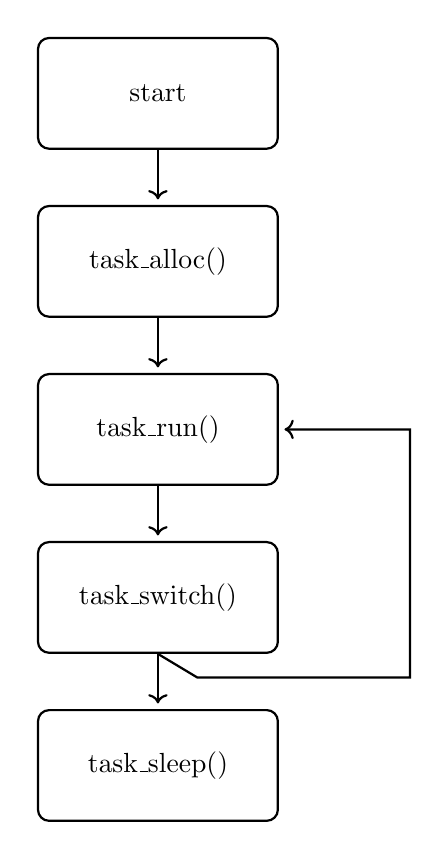
\begin{tikzpicture}
      [auto,
      block/.style={rectangle, draw=black, thick,
      text width=8em,align=center, rounded corners,
      minimum height=4em},
      blank/.style={},
      line/.style={draw, thick, shorten >=2pt, ->}]
    
      \matrix [column sep=5mm,row sep=7mm]
      {
        \node [block] (start) {start}; & \\
        \node [block] (alloc) {task\_alloc()}; & \\
        \node [block] (run)   {task\_run()}; & 
        \node [blank] (blank) {}; \\
        \node [block] (switch) {task\_switch()}; \\ 
        \node [block] (sleep) {task\_sleep()}; & \\
      };
      \begin{scope}[every path/.style=line]
        \path (start) -- (alloc);
        \path (alloc) -- (run);
        \path (run) -- (switch);
        \path (switch.south) -- ++(5mm,-3mm)  -- ++(27mm,0) |- node {} (run);
        \path (switch) -- (sleep);
      \end{scope}
      
      \end{tikzpicture}
    
    \end{document}
    
    %%% Local Variables:
    %%% mode: latex
    %%% TeX-master: t
    %%% End:
    